%%%%%%%%%%%%%%%%%%%%%%%%%%%%%%%%%%%%%%%%%
% Short Sectioned Assignment
% LaTeX Template
% Version 1.0 (5/5/12)
%
% This template has been downloaded from:
% http://www.LaTeXTemplates.com
%
% Original author:
% Frits Wenneker (http://www.howtotex.com)
%
% License:
% CC BY-NC-SA 3.0 (http://creativecommons.org/licenses/by-nc-sa/3.0/)
%
%%%%%%%%%%%%%%%%%%%%%%%%%%%%%%%%%%%%%%%%%

%----------------------------------------------------------------------------------------
%	PACKAGES AND OTHER DOCUMENT CONFIGURATIONS
%----------------------------------------------------------------------------------------

\documentclass[paper=a4, fontsize=11pt]{scrartcl} % A4 paper and 11pt font size

\usepackage[T1]{fontenc} % Use 8-bit encoding that has 256 glyphs
\usepackage{fourier} % Use the Adobe Utopia font for the document - comment this line to return to the LaTeX default
\usepackage[english]{babel} % English language/hyphenation
\usepackage{amsmath,amsfonts,amsthm} % Math packages

\usepackage{graphicx}

\usepackage{sectsty} % Allows customizing section commands
\allsectionsfont{\centering \normalfont\scshape} % Make all sections centered, the default font and small caps

\usepackage{subcaption}
\usepackage{pdfpages}
\usepackage{float}
\usepackage{url}
\usepackage{listings}
\usepackage[toc,page]{appendix}

\usepackage{fancyhdr} % Custom headers and footers
\pagestyle{fancyplain} % Makes all pages in the document conform to the custom headers and footers
\fancyhead{} % No page header - if you want one, create it in the same way as the footers below
\fancyfoot[L]{} % Empty left footer
\fancyfoot[C]{} % Empty center footer
\fancyfoot[R]{\thepage} % Page numbering for right footer
\renewcommand{\headrulewidth}{0pt} % Remove header underlines
\renewcommand{\footrulewidth}{0pt} % Remove footer underlines
\setlength{\headheight}{13.6pt} % Customize the height of the header

\numberwithin{equation}{section} % Number equations within sections (i.e. 1.1, 1.2, 2.1, 2.2 instead of 1, 2, 3, 4)
\numberwithin{figure}{section} % Number figures within sections (i.e. 1.1, 1.2, 2.1, 2.2 instead of 1, 2, 3, 4)
\numberwithin{table}{section} % Number tables within sections (i.e. 1.1, 1.2, 2.1, 2.2 instead of 1, 2, 3, 4)

\setlength\parindent{0pt} % Removes all indentation from paragraphs - comment this line for an assignment with lots of text

%----------------------------------------------------------------------------------------
%	TITLE SECTION
%----------------------------------------------------------------------------------------

\newcommand{\horrule}[1]{\rule{\linewidth}{#1}} % Create horizontal rule command with 1 argument of height

\title{	
\normalfont \normalsize 
\textsc{Bonn-Rhein-Sieg University of Applied Sciences} \\ [25pt] % Your university, school and/or department name(s)
\horrule{0.5pt} \\[0.4cm] % Thin top horizontal rule
\huge Scientific Experimentation and Evaluation\\
- Assignment 09 - \\ 
% The assignment title
Handwritten Data Recognition
\horrule{2pt} \\[0.5cm] % Thick bottom horizontal rule
}

\author{Mazin Eltayeb, Bastian Lang} % Your name

\date{\normalsize\today} % Today's date or a custom date

\begin{document}

\maketitle % Print the title

\tableofcontents
\newpage

\section{Abstract}
This report describes how we applied a machine learning technique to the task of recognizing handwritten digits. It presents our approach, analyses the results and compares them to the results of others that have applied some ML techniques to this task as well.

\section{The Data}
The MNIST dataset is a collection of 70000 images representing handwritten digits ranging from 0 to 9.
The dataset is divided into a training and a test set.
The training set consists of 60000 single images and the test set of 10000 images.
Each image is stored as a 784 row vector, where each vector represents 28x28 pixels.
An example can be seen in figure \ref{fig:sample}.

\begin{figure}[H]
	\centering
	
\includegraphics[width = 0.6\linewidth]{./sample.jpg}
	\caption{Sample Image from MNIST dataset}
	\label{fig:sample}
\end{figure}

\section{Approach}
To classify the handwritten data we used a multilayer perceptron and trained it using the backpropagation of error algorithm. We used the implementation of David Stutz (davidstutz.de) and adjusted the parameters to our needs.
The MLP uses 784 inputs, 700 hidden neurons in its hidden layer and ten outputs - one for each digit.
As the activation function we used a locistic sigmoid:
\[ y = \frac{1}{1+exp(-x)}\]
We set the learning rate to 0.1. The training was done for 500 epochs, where in every epoch we presented 100 randomly chosen samples from the training set and computed the error over the whole batch to adjust the weights.\\
We trained MLP with this settings 50 times and computed its mean and best performance. The results can be seen in section \ref{sec:results}.

\section{Results}
\label{sec:results}

On average the MLP was able to classify 91.91\% correctly. In the best run the performance was about 92.5\%. Figure \ref{fig:pie} visualizes the average performance of the network. The mean error progression while training can be seen in figure \ref{fig:error}. The gradient of the error curve in the figure suggests that continuing the training could possibly lead to an even smaller error. 

\begin{figure}[H]
	\centering
	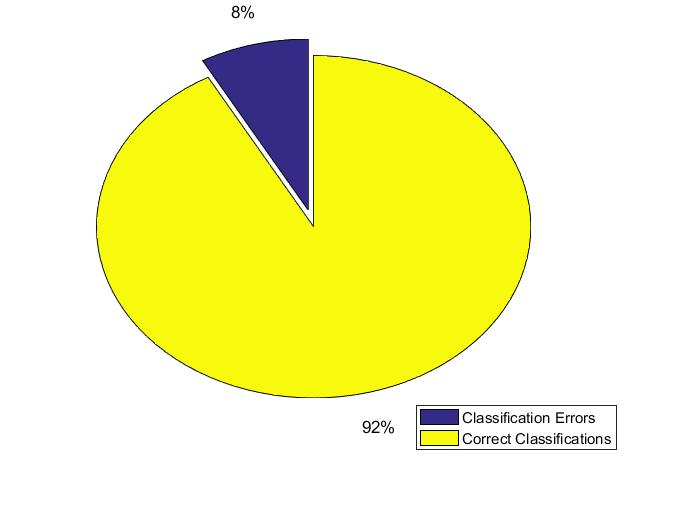
\includegraphics[width = 0.6\linewidth]{./pieChart.jpg}
	\caption{Pie Chart of the Quality of the Classification}
	\label{fig:pie}
\end{figure}

\begin{figure}[H]
	\centering
	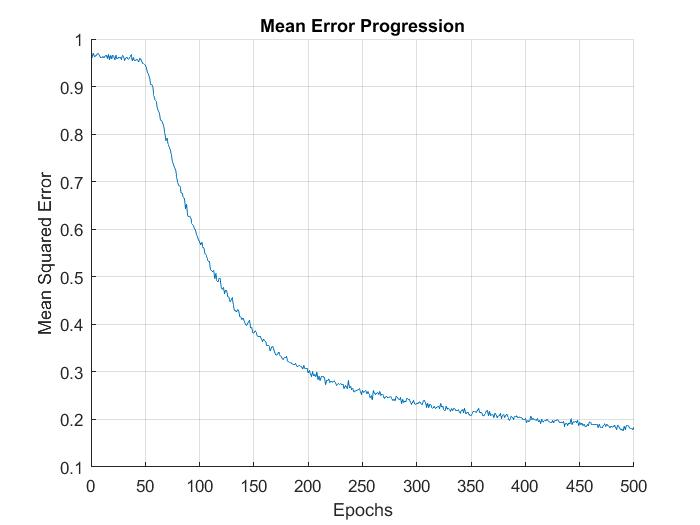
\includegraphics[width = 0.6\linewidth]{./errorProgression.jpg}
	\caption{Error Progression While Training}
	\label{fig:error}
\end{figure}

In table \ref{tab:confusion} and figure \ref{fig:confusion} the confusion matrix of one of the nets can be seen. About 63 times an 8 was mistaken for a 10. About 40 times a 6 for a 9, a 10 for a 5 or a 6 for a 4.

\begin{table}[H]
\centering
\caption{Confusion Matrix}
\label{tab:confusion}
\begin{tabular}{|l||llllllllll|}
\hline
classified\textbackslash real & 0 & 1 & 2 & 3 & 4 & 5 & 6 & 7 & 8 & 9 \\ \hline\hline
0 & 945 & 0 & 4 & 1 & 1 & 8 & 10 & 3 & 4 & 6 \\ \hline
1 & 0 & 1102 & 0 & 0 & 3 & 2 & 3 & 18 & 5 & 7 \\ \hline
2 & 2 & 2 & 952 & 21 & 5 & 2 & 4 & 29 & 4 & 0 \\ \hline
3 & 2 & 6 & 9 & 923 & 0 & 37 & 0 & 4 & 12 & 8 \\ \hline
4 & 0 & 1 & 13 & 1 & 916 & 9 & 11 & 14 & 11 & 44 \\ \hline
5 & 13 & 2 & 3 & 21 & 0 & 761 & 11 & 1 & 14 & 15 \\ \hline
6 & 12 & 5 & 12 & 4 & 11 & 18 & 914 & 0 & 11 & 1 \\ \hline
7 & 1 & 1 & 7 & 4 & 1 & 6 & 0 & 894 & 2 & 3 \\ \hline
8 & 5 & 16 & 28 & 24 & 9 & 41 & 5 & 2 & 900 & 15 \\ \hline
9 & 0 & 0 & 4 & 11 & 36 & 8 & 0 & 63 & 11 & 910 \\ \hline
\end{tabular}
\end{table}

\begin{figure}[H]
	\centering
	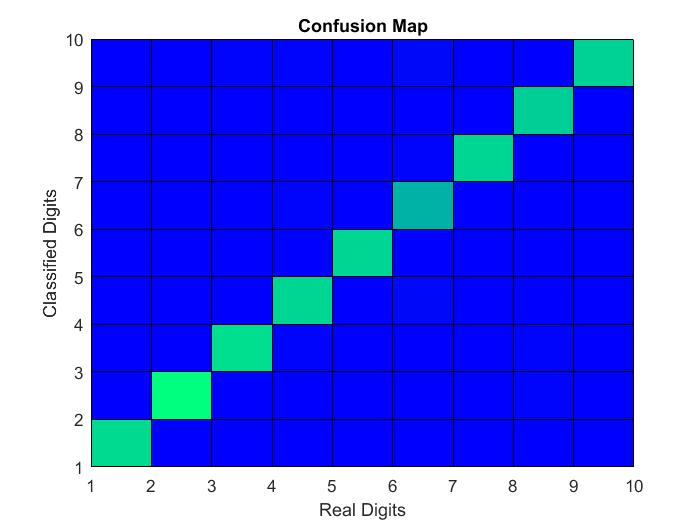
\includegraphics[width = 0.6\linewidth]{./confusion.jpg}
	\caption{Graphical Confusion Matrix of Classifications}
	\label{fig:confusion}
\end{figure}

\section{Comparison}
We compared the accuracies of the MLP approach with two other approaches. One approach was to use PCA to reduce the dimensionality of the problem and then use an SVM to classify the images. The other approach also used an SVM for classification, but it used a method named \textit{Sparse Coding} for preprocessing.\\
The results can be seen in table \ref{tab:comparison}.
Using PCA in combination with SVM performed best and significantly outperformed the other methods.
The MLP achieved a slighty better performance than the sparse coding approach.


\begin{table}[H]
\centering
\caption{Accuracies of Different Approaches}
\label{tab:comparison}
\begin{tabular}{l|lll}
Method & MLP & Sparse Coding + SVM & PCA + SVM \\ \hline
Average Accuracy & 91.91\% & 89.92\% & ~98\%
\end{tabular}
\end{table}

\section{Conclusion}
Using PCA in combination with SVM seems to be the best method to use here. On the other hand some more information are missing to be sure about it. No runtime or memory usage analysis could be done due to lack of information.\\
For the PCA/SVM approach no information about the number of performed experiments were available, so it may be possible that this result is an outlier. For the Sparse Coding approach the average accuracy is based on three runs only, which is also not enough to make a statistically sound statement.



\end{document}